% Build from this directory:
% latex -interaction=nonstopmode -halt-on-error stoer-wagner-1.tex
% dvisvgm --no-fonts --exact --bbox=papersize stoer-wagner-1.dvi -o stoer-wagner-1.svg
\documentclass[tikz,border=5pt]{standalone}
\definecolor{graphline}{HTML}{294760}
\definecolor{regiona}{HTML}{D5EEF3}
\definecolor{regionb}{HTML}{FFF1B8}
\begin{document}
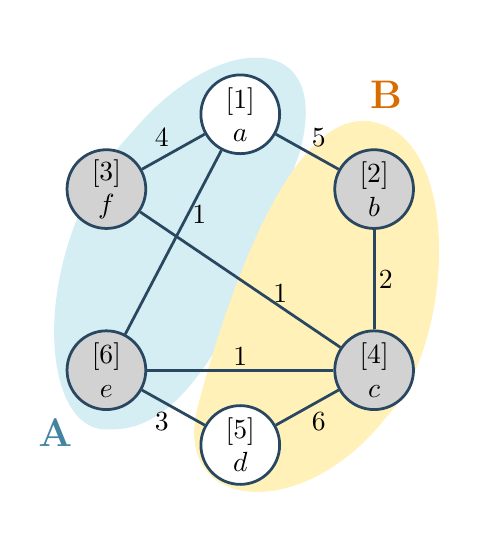
\begin{tikzpicture}[
  vertex/.style={circle,draw=graphline,line width=1pt,fill=white,
    minimum size=10mm,inner sep=1pt,align=center,font=\normalsize},
  active/.style={fill=gray!35},
  edge/.style={draw=graphline,line width=1pt},
  weight/.style={inner sep=1.2pt,font=\normalsize}
]
  % The cut separates {a,f,e} from {b,c,d}. Consecutive additions switch
  % sides at b, f, c, e, which are exactly the gray (active) vertices.
  \fill[regiona] (-1.65,-1.6)
    .. controls (-2.6,-1.7) and (-2.7,.8) .. (-1.35,2.2)
    .. controls (-.3,3.45) and (1.2,3.5) .. (.75,1.9)
    .. controls (.3,.65) and (-.45,-1.65) .. (-1.65,-1.6);
  \fill[regionb] (1.7,2.3)
    .. controls (2.85,2.05) and (2.7,-.55) .. (1.85,-1.45)
    .. controls (.8,-2.8) and (-.85,-2.65) .. (-.55,-1.35)
    .. controls (-.25,-.2) and (.6,2.55) .. (1.7,2.3);
  \node[font=\Large\bfseries,text=cyan!60!black] at (-2.35,-1.65) {A};
  \node[font=\Large\bfseries,text=orange!85!black] at (1.85,2.65) {B};

  \node[vertex]        (a) at (0,2.4) {$[1]$\\$a$};
  \node[vertex,active] (b) at (1.7,1.45) {$[2]$\\$b$};
  \node[vertex,active] (c) at (1.7,-.85) {$[4]$\\$c$};
  \node[vertex]        (d) at (0,-1.8) {$[5]$\\$d$};
  \node[vertex,active] (e) at (-1.7,-.85) {$[6]$\\$e$};
  \node[vertex,active] (f) at (-1.7,1.45) {$[3]$\\$f$};
  \draw[edge] (a) -- node[weight,above left] {4} (f);
  \draw[edge] (a) -- node[weight,above right] {5} (b);
  \draw[edge] (a) -- node[weight,pos=.35,right] {1} (e);
  \draw[edge] (f) -- node[weight,pos=.7,above] {1} (c);
  \draw[edge] (b) -- node[weight,right] {2} (c);
  \draw[edge] (e) -- node[weight,above] {1} (c);
  \draw[edge] (e) -- node[weight,below left] {3} (d);
  \draw[edge] (c) -- node[weight,below right] {6} (d);
\end{tikzpicture}
\end{document}
